\documentclass[tikz,border=4pt]{standalone}
\usepackage[T1]{fontenc}
\usepackage[utf8]{inputenc}
\usepackage{tikz}
\usetikzlibrary{arrows.meta,positioning,calc,fit}

% ------------------------------------------------------------
% Palette consistent with the approved TFM / defense graphics
% ------------------------------------------------------------
\definecolor{archdark}{HTML}{263142}
\definecolor{archslate}{HTML}{64748B}
\definecolor{archlight}{HTML}{F8FAFC}
\definecolor{archmuted}{HTML}{EEF2F7}
\definecolor{subsysTUFill}{HTML}{DCEAF7}
\definecolor{subsysFUFill}{HTML}{DDEED8}
\definecolor{subsysATMFill}{HTML}{F7E6B8}
\definecolor{subsysACTFill}{HTML}{F3D8DE}
\definecolor{subsysELECFill}{HTML}{E4DDF2}
\definecolor{subsysCTRLFill}{HTML}{D6ECEF}
\definecolor{subsysEXPFill}{HTML}{E5E7EB}
\definecolor{flexColor}{HTML}{C2185B}
\definecolor{extColor}{HTML}{007C91}

\tikzset{
  >={Latex[length=2.3mm,width=1.45mm]},
  flow/.style={->, draw=archdark, line width=0.9pt},
  soft/.style={draw=archdark, rounded corners=3pt, line width=0.8pt,
               fill=white, text=archdark, font=\small\sffamily,
               inner xsep=4pt, inner ysep=3pt, align=center},
  chip/.style={draw=archdark!35, rounded corners=3pt, line width=0.7pt,
               text=archdark, font=\scriptsize\bfseries\sffamily,
               inner xsep=5pt, inner ysep=3pt, align=center},
  label/.style={font=\scriptsize\sffamily, text=archdark, align=center},
  miniTitle/.style={font=\bfseries\small\sffamily, text=archdark, align=center},
  person/.style={draw=archdark, line width=0.9pt, line cap=round, line join=round}
}

\begin{document}
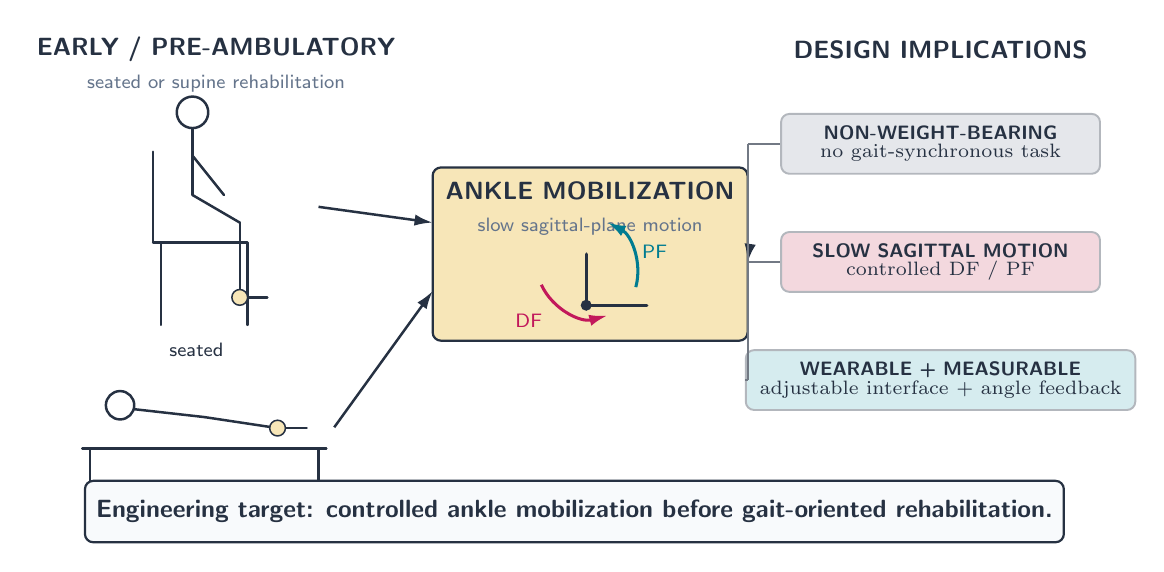
\begin{tikzpicture}[font=\sffamily]

% ------------------------------------------------------------
% LEFT: early-rehabilitation postures
% ------------------------------------------------------------
\node[miniTitle] at (2.25,6.05) {EARLY / PRE-AMBULATORY};
\node[label, text=archslate] at (2.25,5.62) {seated or supine rehabilitation};

% Seated icon
\begin{scope}[shift={(1.2,3.75)}]
  % chair
  \draw[person] (0.25,-0.15) -- (1.45,-0.15) -- (1.45,-1.20);
  \draw[person] (0.35,-0.15) -- (0.35,-1.20);
  \draw[person] (0.25,-0.15) -- (0.25,1.00);
  % person
  \draw[person] (0.75,1.50) circle (0.20);
  \draw[person] (0.75,1.30) -- (0.75,0.45);
  \draw[person] (0.75,0.95) -- (1.15,0.45);
  \draw[person] (0.75,0.45) -- (1.35,0.10);
  \draw[person] (1.35,0.10) -- (1.35,-0.85);
  \draw[person] (1.35,-0.85) -- (1.70,-0.85);
  \fill[subsysATMFill, draw=archdark, line width=0.55pt] (1.35,-0.85) circle (0.10);
  \node[label, anchor=north] at (0.8,-1.30) {seated};
\end{scope}

% Supine icon
\begin{scope}[shift={(0.55,1.18)}]
  % bed
  \draw[person] (0,-0.20) -- (3.10,-0.20);
  \draw[person] (0.10,-0.20) -- (0.10,-0.72);
  \draw[person] (3.00,-0.20) -- (3.00,-0.72);
  % person
  \draw[person] (0.48,0.35) circle (0.18);
  \draw[person] (0.66,0.30) -- (1.55,0.20);
  \draw[person] (1.55,0.20) -- (2.48,0.06);
  \draw[person] (2.48,0.06) -- (2.85,0.06);
  \fill[subsysATMFill, draw=archdark, line width=0.55pt] (2.48,0.06) circle (0.10);
  \node[label, anchor=north] at (1.55,-0.78) {supine};
\end{scope}

% ------------------------------------------------------------
% CENTER: ankle mobilization concept
% ------------------------------------------------------------
\node[soft, fill=subsysATMFill, minimum width=4.0cm, minimum height=2.20cm] (ankle) at (7.0,3.45) {};
\node[miniTitle] at (7.0,4.25) {ANKLE MOBILIZATION};
\node[label, text=archslate] at (7.0,3.80) {slow sagittal-plane motion};

% stylized tibia-foot
\draw[person, line width=1.2pt] (6.95,3.45) -- (6.95,2.80);
\draw[person, line width=1.2pt] (6.95,2.80) -- (7.72,2.80);
\fill[archdark] (6.95,2.80) circle (0.07);

% DF/PF curved arrows
\draw[->, draw=flexColor, line width=1.1pt] (6.38,3.06) arc[start angle=205,end angle=285,radius=0.72];
\draw[->, draw=extColor, line width=1.1pt] (7.58,3.03) arc[start angle=-15,end angle=62,radius=0.72];
\node[label, text=flexColor] at (6.22,2.60) {DF};
\node[label, text=extColor] at (7.82,3.48) {PF};

% left-to-center convergence
\draw[flow] (3.55,4.05) -- (5.0,3.85);
\draw[flow] (3.75,1.25) -- (5.0,2.98);

% ------------------------------------------------------------
% RIGHT: design implications
% ------------------------------------------------------------
\node[miniTitle] at (11.45,6.05) {DESIGN IMPLICATIONS};

\node[chip, fill=subsysEXPFill, minimum width=4.05cm, minimum height=0.76cm] (nw) at (11.45,4.85)
{NON-WEIGHT-BEARING\\[-0.5mm]\normalfont\scriptsize no gait-synchronous task};
\node[chip, fill=subsysACTFill, minimum width=4.05cm, minimum height=0.76cm] (slow) at (11.45,3.35)
{SLOW SAGITTAL MOTION\\[-0.5mm]\normalfont\scriptsize controlled DF / PF};
\node[chip, fill=subsysCTRLFill, minimum width=4.05cm, minimum height=0.76cm] (meas) at (11.45,1.85)
{WEARABLE + MEASURABLE\\[-0.5mm]\normalfont\scriptsize adjustable interface + angle feedback};

% One clean connection to the grouped design implications
\coordinate (bus) at (9.0,3.35);
\draw[flow] (ankle.east) -- (bus);
\draw[draw=archdark!65, line width=0.8pt] (9.0,1.85) -- (9.0,4.85);
\draw[draw=archdark!65, line width=0.8pt] (9.0,4.85) -- (nw.west);
\draw[draw=archdark!65, line width=0.8pt] (9.0,3.35) -- (slow.west);
\draw[draw=archdark!65, line width=0.8pt] (9.0,1.85) -- (meas.west);

% Bottom takeaway band
\node[soft, fill=archlight, minimum width=12.0cm, minimum height=0.78cm,
      font=\small\bfseries\sffamily] at (6.8,0.18)
{Engineering target: controlled ankle mobilization before gait-oriented rehabilitation.};

\end{tikzpicture}
\end{document}
